\documentclass{statsoc}
% \usepackage{mathtime}
\usepackage{ccfonts,eulervm}
% \usepackage[T1]{fontenc}
% \usepackage[lite]{belleek}
% \fontfamily{belleek}
% \usepackage[math]{belleek}
% \usepackage{concretemath-fonts}

% ---------------------------------------------------------------------------------------------------------------------------------
% The statsoc style file is broken?
% I have copied this code straight from stack overflow
% https://tex.stackexchange.com/questions/351768/problem-with-statsoc-class-and-pdflatex
\usepackage{geometry}

\geometry{
  textwidth=33pc,
  textheight=\dimexpr48\baselineskip+\topskip\relax,
  marginparsep=11pt,
  marginparwidth=107pt,
  footnotesep=6.65pt,
  headheight=9pt,
  headsep=9pt,
  footskip=30pt,
}
% ---------------------------------------------------------------------------------------------------------------------------------

% \usepackage{natbib}
\bibliographystyle{chicago}

% TODO: Are we, in this setting, immune to confounders?  We are removing
%       all bi-directional edges, so it seems likely that we are?  Can we state
%       any theorem about this?

%% bibliography stuff -- this needs come before the preamble inclusion
\usepackage{enumitem}
\usepackage{etex,etoolbox}
\usepackage{hyperref}
\usepackage{fullpage}
\setlength{\marginparwidth}{2cm}
\usepackage{todonotes}

\def\gc{\overset{\text{GC}}{\rightarrow}}  % Granger causality arrow
\def\ngc{\overset{\text{GC}}{\nrightarrow}}  % Negated Granger causality arrow
\def\pwgc{\overset{\text{PW}}{\rightarrow}}  % Pairwise Granger causality arrow
\def\npwgc{\overset{\text{PW}}{\nrightarrow}}  % Negated pairwise Granger causality arrow
\def\te{\overset{\mathcal{T}}{\rightarrow}}  % Transfer entropy arrow
\def\gcg{\mathcal{G}}  % Granger-causality graph
\def\gcge{\mathcal{E}}  % Graph edges
\def\VAR{\mathsf{VAR}}  % VAR(p) model
\def\B{\mathsf{B}}  % Filter B
\def\wtB{\widetilde{\B}}  % General filter B
\def\A{\mathsf{A}}  % Filter A
\def\H{\mathcal{H}}  % Hilbert space

\newcommand{\linE}[2]{\hat{\E}[#1\ |\ #2]}  % Linear projection
\newcommand{\linEerr}[2]{\xi[#1\ |\ #2]}  % Error of linear projection
\newcommand{\pa}[1]{pa(#1)}  % Parents of a node
\newcommand{\anc}[1]{\mathcal{A}(#1)}  % Ancestors of a node
\newcommand{\ancn}[2]{\mathcal{A}_{#1}(#2)}  % nth ancestors of a node
\newcommand{\gpn}[2]{gp_{#1}(#2)}  % nth generation grandparents
\newcommand{\wtalpha}[2]{\widetilde{\alpha}(#1, #2)}  % Some notation for lem:pwgc_anc
\newcommand{\dist}[2]{\mathsf{d}(#1, #2)}  % Distance between things
\newcommand{\gcgpath}[2]{#1 \rightarrow \cdots \rightarrow #2}  % A shorter path command

% \usepackage{fullpage}
\usepackage{framed}

% Figures
\usepackage{graphicx}
\usepackage{caption}  % This is not recommended?
\usepackage{subcaption}
% \usepackage{wrapfig}
% \usepackage{svg}

% Math packages, theorem definitions and numbering
\usepackage{amsmath}
\usepackage{amssymb}
% \usepackage{amsthm}
% \usepackage{mathrsfs} % Fancy scripted font
% \usepackage{bm}  % Bold math

% Misc packages
\usepackage[linesnumbered, ruled, vlined]{algorithm2e}
\usepackage{algorithm2e} %{algorithm} environment
\usepackage{soul}  % \hl highlighting
\usepackage{color}
\usepackage{mathtools}  % For my \ceil function

% Theorems (with italics)
% \theoremstyle{plain}  % Style definition removes italics
\newtheorem{theorem}{Theorem}
\newtheorem{corollary}{Corollary}
\newtheorem{proposition}{Proposition}
\newtheorem{lemma}{Lemma}

% \theoremstyle{definition}
\newtheorem{remark}{Remark}
\newtheorem{definition}{Definition}
\newtheorem{example}{Example}
\newtheorem{assumptions}{Assumptions}

% keywords
\providecommand{\keywords}[1]{\textbf{\textit{Keywords---}} #1}

% General
\def\defeq{\overset{\Delta}{=}}  % Equal with triangle
\def\cl{\mathsf{cl\ }}  % Closure
\newcommand{\sgn}[1]{\mathsf{sgn}(#1)}  % sign function

% Calculus
\def\d{\mathsf{d}}  % Differential operator

% Functions
\def\ln{\mathsf{ln\ }}  % Natural logarithm
\DeclarePairedDelimiter{\ceil}{\lceil}{\rceil}  % Ceiling

% Probability
\def\H{\mathcal{H}}  % Hilbert space
\def\E{\mathbb{E}}  % Expectation
\def\Var{\text{Var}}  % Variance
\def\P{\mathbb{P}}  % Probability Measure
\def\F{\mathcal{F}}  % A sigma algebra
\def\sX{\mathcal{X}}  % Another sigma algebra
\def\KL{\mathbf{D}_{KL}}  % KL divergence
\def\bF{\mathbf{F}}  % Whole F-meas space

% Standard sets
\def\Z{\mathbb{Z}}  % Set of integers
\def\R{\mathbb{R}}  % Set of real numbers
\def\C{\mathbb{C}}  % Set of complex numbers
\def\N{\mathbb{N}}  % Set of natural numbers
\def\ball{\mathbb{B}}  % Open ball
\def\clball{\overline{\ball}}  % Closed ball

% Linear algebra
\def\rk{\mathsf{rk }}  % The rank
\def\tr{\mathsf{tr }}  % The trace
\def\T{\mathsf{T}}  % Transpose notation
\def\c{\mathsf{c}}  % complement
\def\dg{\mathsf{dg }}   %  Diagonal vector of a matrix
\def\Dg{\mathsf{Dg }}   %  Diagonal matrix from a vector
\def\ind{\mathbf{1}}  % Ones vector or indicator
\def\matvec{\textbf{vec}}  % Vector operator
\def\<{\langle}  % < Inner product
\def\>{\rangle}  % > Inner product
\newcommand{\inner}[2]{\langle #1, #2 \rangle}  % Inner product
\newcommand{\innerT}[2]{#1^\T #2}  % Inner product for finite vectors

\graphicspath{{../figures/}}

\title{Graph Topological Aspects of Granger Causal Network Learning}
\author[Author 1 {\it et al.}]{R. J. Kinnear}
\address{
  University of Waterloo,
  Waterloo,
  Canada.}
\email{Ryan@Kinnear.ca}

\author{R. R. Mazumdar}
\address{
  University of Waterloo,
  Waterloo,
  Canada.}

\begin{document}

\abstract{We study Granger-causality in the context of wide-sense
  stationary time series, where our focus is on the topological
  aspects of the underlying causality graph.  We establish sufficient
  conditions (in particular, we develop the notion of a ``strongly
  causal'' graph topology) under which the true causality graph can be
  recovered via pairwise causality testing alone, and provide examples
  from the gene regulatory network literature suggesting that our
  concept of a strongly causal graph may be applicable to this field.}

\keywords{causality graph, gene regulatory networks,
  Granger-causality, network learning, time series, vector
  autoregression}

\paragraph{Acknowledgement}

We acknowledge the support of the Natural Sciences and Engineering Research Council of Canada (NSERC), [funding reference number 518418-2018].  Cette recherche a été financée par le Conseil de recherches en sciences naturelles et en génie du Canada (CRSNG), [numéro de référence 518418-2018].

\clearpage

% \tableofcontents
\clearpage

\section{Introduction and Review}
\label{sec:introduction}
In this paper we study the notion of Granger-causality
\cite{granger1969investigating} \cite{Granger1980329} as a means of
uncovering an underlying causal structure in multivariate time series.
Though the underlying causality graph cannot be observed directly, we
will infer it's presence as a latent structure among our observed time
series data.  This notion is leveraged in a variety of applications
e.g. in Neuroscience as a means of recovering interactions amongst
brain regions \cite{bressler2011wiener}, \cite{anna_paper2008},
\cite{david2008identifying}; in the study of the dependence and
connectedness of financial institutions \cite{NBERw16223}; gene
expression networks \cite{Fujita2007},
\cite{methods_for_inferring_gene_regulatory_networks_from_time_series_expression_data},
\cite{grouped_graphical_granger_modelling_for_gene_expression_regulatory_networks_discovery},
\cite{discovering_graphical_Granger_causality_using_the_truncating_lasso_penalty};
and power system design \cite{Misyrlis2016450}, \cite{yuan2014root}.

Granger-causality can generally be formulated by searching for the
``best'' graph structure consistent with observed data, which is in
general an extremely challenging problem (i.e. it may be framed as a
best subset selection problem, see \cite{bss_mio},
\cite{hastie_bss_comp}), moreover, the comparison of quality between
different structures, and hence the notion of ``best'' needs
qualification.  In applications where we are interested merely in
minimizing the mean squared error of a linear one-step-ahead
predictor, then we will be satisfied with an entirely dense graph of
connections, since each edge can only serve to reduce estimation
error.  However, since the number of edges scales quadratically in $n$
(the number of nodes) it becomes imperative to infer a sparse
causality graph for large systems, both to avoid overfitting observed
data, as well as to aid the interpretability of the results.

A fairly early approach to the problem in the context of large systems
is provided by \cite{bach2004learning}, where the authors apply a
local search heuristic to the Whittle likelihood with an AIC
penalization.  The local search heuristic where at each iteration an
edge is either added, removed, or reversed is a common approach to
combinatorial optimization due to it's simplicity, but is liable to
get stuck in shallow local minima.

A second and wildly successful heuristic is the LASSO regularizer
\cite{tibshirani1996regression}, which can be understood as a natural
convex relaxation to penalizing the count of the non-zero edges.  The
LASSO enjoys fairly strong theoretical guarantees
\cite{wainwright2009sharp}, extending largely to the case of
stationary time series data with a sufficiently fast rate of
dependence decay \cite{basu2015} \cite{wong2016lasso}
\cite{autoregressive_process_modelling_via_the_lasso_procedure}, and
variations on the LASSO have been applied in a number of different
time series contexts as well as Granger-causality
\cite{DBLP:journals/corr/HallacPBL17} \cite{haufe2008sparse}
\cite{bolstad2011causal} \cite{he2013stationary}
\cite{grouped_graphical_granger_modelling_for_gene_expression_regulatory_networks_discovery}.
One of the key improvements to the original LASSO algorithm is the
adaptive (i.e. weighted) ``adaLASSO'' \cite{adaptive_lasso_zou2006},
for which oracle results (i.e. asymptotic support recovery) are
established under less restrictive conditions than for the vanilla
LASSO.  We study a novel perspective on the problem by establishing
conditions under which simple \textit{pairwise} Granger-causality
tests are sufficient to recover the entire graph.

%   Prior assumptions
% on the \textit{topology} of the underlying Granger-causality graph can
% result in tests more powerful than more generally applicable
% algorithms, and we provide examples from the literature where
% simplifying topological assumptions may be met.

\subsection{Contributions}
In the context of time series data, sparsity assumptions remain
important, but there is significant additional structure that may
arise as a result of considering the topology of the underlying
Granger-causality graph, which to our knowledge remains largely
unexplored.  The focus of this paper is to shed light on some of these
topological questions, in particular, we study a particularly simple
notion of causality graph topology which we term ``strongly causal''
and show that stationary times series whose underlying causality graph
has this structure satisfy natural intuitive notions of ``information
flow'' through the graph.  Moreover, we show that such graphs are
perfectly recoverable with only \textit{pairwise} Granger-causality
tests, which would otherwise suffer from serious confounding problems.
Aside from being an interesting theoretical perspective, prior
assumptions about the underlying graph (similarly to sparsity
assumptions) can greatly improve upon the statistical power of
causality graph recovery algorithms when the assumptions are met.

In the case of gene expression networks, we show examples from the
literature which suggest our concept of a ``strongly causal graph''
topology may have application in this field (see Section
\ref{sec:strongly_causal_graphs}).

The principle contributions of this paper are as follows: firstly, in
section \ref{sec:theory} we study \textit{pairwise} Granger-causality
relations, providing novel theorems connecting the structure of the
causality graph to the pairwise ``causality flow'' in the system, as
well as an interpretation in terms of the graph topology of the
sparsity pattern of matrices arising in the Wold decomposition,
generalizing in some sense the notion of ``feedback-free'' processes
studied by \cite{caines1975feedback} in close connection with
Granger-causality.  We establish sufficient conditions (sections
\ref{sec:strongly_causal_graphs}, \ref{sec:persistent_systems}) under
which a fully conditional Granger-causality graph can be recovered
from pairwise tests alone (sec \ref{sec:pairwise_algorithm}).  We
report \hl{elsewhere}\todo{where?  Or can I fit in a brief summary?}
the results of extensive finite sample simulations as well as an
application to EEG data, where in addition we summarize appropriate
methods for hypothesis testing, model order selection, computationally
efficient estimations, and error rate controls in practice.  Our
simulation results establish significant potential for improvement
over existing methods.  Concluding remarks on further open problems
and extentions are provided in Section \ref{sec:conclusion}.

\section{Graph Topological Aspects of Granger-causality}
\label{sec:theory}
\subsection{Formal Setting}
Consider the space $L_2(\Omega)$, the usual Hilbert space of finite
variance random variables over a probability space
$(\Omega, \mathcal{F}, \mathbb{P})$ having inner product
$\inner{x}{y} = \E[xy]$.  We will work with a discrete time and
wide-sense stationary (WSS) $n$-dimensional vector valued process
$x(t)$ (with $t \in \Z$) where the $n$ elements take values in $L_2$.
We suppose that $x(t)$ has zero mean, $\E x(t) = 0$, and has
absolutely summable matrix valued covariance sequence
$R(\tau) \overset{\Delta}{=} \E x(t)x(t - \tau)^\T$, and an absolutely continuous
spectral density.

We will also work frequently with the spaces spanned by the values of
such a process

\begin{equation}
  \label{eq:hilbert_space_defn}
  \begin{aligned}
    % \H^x &= \cl \{\sum_{\tau = -T}^T a_\tau^\T x(t - \tau)\ |\ a_\tau \in \R^n, T \in \N\} \subseteq L_2(\Omega),\\
    \H_t^x &= \cl \{\sum_{\tau = 0}^p a_\tau^\T x(t - \tau)\ |\ a_\tau \in \R^n, p \in \N\} \subseteq L_2(\Omega)\\
    H_t^x &= \{a x(t)\ |\ a \in \R\} \subseteq L_2(\Omega),
  \end{aligned}
\end{equation}

where the closure is naturally in mean-square.  We will often omit the
superscript $x$ which should be clear from context.  Evidently these
spaces are separable, and as closed subspaces of a Hilbert space they
are themselves Hilbert.  We will denote the spaces generated in
analogous ways by particular components of $x$ as e.g.
$\H_t^{(i, j)}$, $\H_t^{i}$ or by all but particular components as
$\H_t^{-j}$.

As a consequence of the Wold decomposition theorem \cite{lindquist},
every WSS sequence has the moving average $MA(\infty)$
representation

\begin{equation}
\label{eqn:wold}
  x(t) = c(t) + \sum_{\tau = 0}^\infty A(\tau) v(t - \tau),
\end{equation}

where $c(t)$ is a purely deterministic sequence$v(t)$ is an
uncorrelated sequence and $A(0) = I$.  We will assume that $c(t) = 0$.
We additionally require that this representation can be inverted to
yield the $\VAR(\infty)$ form

\begin{equation}
  \label{eqn:ar_representation}
  x(t) = \sum_{\tau = 1}^\infty B(\tau) x(t - \tau) + v(t).
\end{equation}

The equations (\ref{eqn:wold}), (\ref{eqn:ar_representation}) can be
represented as $x(t) = \A(z)v(t) = \B(z)x(t) + v(t)$ via the action
(convolution) of the operators (LTI filters)
$\A(z) \defeq \sum_{\tau = 0}^\infty A(\tau)z^{-\tau}$ and
$\B(z) \defeq \sum_{\tau = 1}^\infty B(\tau)z^{-\tau}$ where the
operator $z^{-1}$ is the back shift operator acting on
$\ell_2^n(\Omega, \mathcal{F}, \mathbb{P})$, that is:

\begin{equation}
  \label{eqn:filter_action}
  \B_{ij}(z)x_j(t) \defeq \sum_{\tau = 1}^\infty B_{ij}(\tau)x_j(t - \tau).
\end{equation}

Finally, we have the inversion formula

\begin{equation}
  \label{eqn:lsi_inversion}
  \A(z) = (I - \B(z))^{-1} = \sum_{k = 0}^\infty \B(z)^k.
\end{equation}

The aforementioned assumptions are quite weak.  The strongest
assumption we require is finally that $\Sigma_v$ is a diagonal matrix,
which is referred to as a lack of instantaneous feedback in $x(t)$.
We formally state our setup as a definition, which is the setup for
the remainder of the paper:

\begin{definition}[Basic Setup]
  \label{def:basic_setup}
  The process $x(t)$ is an $n$ dimensional wide sense stationary
  process having invertible $\VAR(\infty)$ representation
  \eqref{eqn:ar_representation} where $v(t)$ is sequentially
  uncorrelated and has a diagonal covariance matrix.  The $MA(\infty)$
  representation of equation \eqref{eqn:wold} has $c(t) = 0$ and
  $A(0) = I$.
\end{definition}

\subsection{Granger Causality}

\begin{definition}[Granger Causality]
  \label{def:granger_causality}
  For the WSS series $x(t)$ satisfying the assumptions of Definition
  \ref{def:basic_setup} we will say that component $x_j$
  \textit{Granger-Causes} (GC) component $x_i$ (with respect to $x$)
  and write $x_j \gc x_i$ if given Hilbert spaces $\H_{t - 1}$,
  $\H^{-j}_{t - 1}$

\begin{equation}
  \linEerr{x_i(t)}{\H_{t - 1}} < \linEerr{x_i(t)}{\H^{-j}_{t - 1}},
\end{equation}

where $\xi[x \ |\ \H] = \E (x - \linE{x}{\H})^2$ is the mean squared
estimation error and $\linE{x}{\H} = \text{proj}_{\H}(x)$ denotes the
(unique) projection onto the Hilbert space $\H$.
\end{definition}

This notion captures the idea that the process $x_j$ provides
information about $x_i$ that is not available from elsewhere.  The
caveat ``with respect to $x$'' is important in that GC relations can
change when components are added to or removed from our collection $x$
of observations, e.g. new GC relations can arise if we remove the
observations of a common cause, and existing GC relations can
disappear if we observe a new mediating series. The notion is closely
related to the information theoretic measure of transfer entropy,
indeed, if the distribution of $v(t)$ is known to be Gaussian then
they are equivalent \cite{barnett2009granger}.

The notion of conditional orthogonality is used throughout, as well as
some equivalent representations for Granger-causality.

\begin{lemma}[\cite{lindquist} Proposition 2.4.2]
  \label{lem:conditional_orthogonality_equivalence}
  Consider three closed subspaces of a Hilbert space $\mathcal{A}$,
  $\mathcal{B}$, $\mathcal{X}$.  The following statements are
  equivalent

  \todo{Do I even use (a) anymore?  I think I can just put the definition of conditional orthogonality into Theorem 1.}

  \begin{enumerate}
    \item{$\mathcal{A} \perp \mathcal{B}\ |\ \mathcal{X}$}
    \item{$\linE{\beta}{\mathcal{A} \vee \mathcal{X}} = \linE{\beta}{\mathcal{X}}\ \forall \beta \in \mathcal{B}$.}
    % \item{$\linE{\beta}{\mathcal{A}} = \linE{\linE{\beta}{\mathcal{X}}}{\mathcal{A}}\ \forall \beta \in \mathcal{B}}$}
    \end{enumerate}

    Where $\mathcal{A} \perp \mathcal{B}\ |\ \mathcal{X}$ denotes
    conditional orthogonality:

    \begin{equation*}
      \inner{a - \linE{a}{\mathcal{X}}}{b - \linE{b}{\mathcal{X}}} = 0\ \forall a \in \mathcal{A}, b \in \mathcal{B}.
    \end{equation*}
\end{lemma}

\begin{theorem}[Granger Causality Equivalences]
  \label{thm:granger_causality_equivalences}
  The following are equivalent:

  \begin{enumerate}
    \item{$x_j \ngc x_i$}
    \item{$\forall \tau \in \N_+\ B_{ij}(\tau) = 0$ i.e. $\B_{ij}(z) = 0$}
    \item{$H_t^{i} \perp \H_{t - 1}^{j}\ |\ \H_{t - 1}^{-j}$}
    \item{$\linE{x_i(t)}{\H_{t - 1}^{-j}} = \linE{x_i(t)}{\H_{t - 1}}$}
  \end{enumerate}
\end{theorem}

\begin{proof}
  % Geweke uses the log of the ratio of the determinants of the residual variances
  % 
  % The equivalence $(1) \iff (3)$ is essentially a restatement of the
  % definition, but is in line with the seminal work of Geweke
  % \cite{geweke1982measurement}, \cite{geweke1984}.

  $(1) \Rightarrow (2)$ follows as a result of the uniqueness of orthogonal
  projection (i.e. the best estimate is necessarily the coefficients
  of the model).  $(2) \Rightarrow (3)$ follows since in computing
  $(y - \linE{y}{\H_{t - 1}^{-j}})$ for $y \in H_t^i$ it is sufficient
  to consider $y = x_i(t)$ by linearity, then since
  $H_{t - 1}^i \subseteq \H_{t - 1}^{-j}$ we have
  $(x_i(t) - \linE{x_i(t)}{\H_{t = 1}^{-j}}) = v_i(t)$ since
  $\B_{ij}(z) = 0$ and $v_i(t) \perp \H_{t - 1}$.  $(3) \iff (4)$ is a result
  of Lemma \ref{lem:conditional_orthogonality_equivalence}.  And,
  $(4) \implies (1)$ follows directly from the Definition.
\end{proof}

\subsection{Granger Causality Graphs}
We establish some graph theoretic notation and terminology, collected
formally in definitions for the reader's convenient reference.

\begin{definition}[Graph Theory Review]
  A \textit{graph} $\gcg = (V, \gcge)$ is simply a
  tuple of sets respectively called \textit{nodes} and \textit{edges}.
  Throughout this paper, we have in all cases
  $V = [n] \defeq \{1, 2, \ldots, n\}$.  We will also focus solely on
  \textit{directed} graphs, where the edges
  $\gcge \subseteq V \times V$ are \textit{ordered} pairs.

  A (directed) \textit{path} (of length $r$) from node $i$ to node
  $j$, denoted $\gcgpath{i}{j}$, is a sequence
  $a_0, a_1, \ldots, a_{r - 1}, a_r$ with $a_0 = i$ and $a_r = j$ such
  that $\forall\ 0 \le k \le r\ (a_k, a_{k + 1}) \in \gcge$, and where
  $(a_k, a_{k - 1})$ are \textit{distinct} for $0 \le k < r$.

  A \textit{cycle} is a path of length $2$ or more between a node and
  itself.  An edge between a node and itself $(i, i) \in \gcge$ (which
  is not a cycle) is referred to as a \textit{loop}.

  A graph $\gcg$ is a \textit{directed acyclic graph} (DAG) if it is a
  directed graph and does not contain any cycles.
\end{definition}

\begin{definition}[Parents, Grandparents, Ancestors]
  A node $j$ is a \textit{parent} of node $i$ if $(j, i) \in \gcge$.
  The set of all $i$'s parents will be denoted $\pa{i}$, and we
  explicitly exclude loops as a special case, that is,
  $i \not\in \pa{i}$ even if $(i, i) \in \gcge$.

  The set of level $\ell$ \textit{grandparents} of node $i$, denoted
  $\gpn{\ell}{i}$, is the set such that $j \in \gpn{\ell}{i}$ if and
  only if there is a \textit{directed path} of length $\ell$ in $\gcg$
  from $j$ to $i$.  Clearly, $\pa{i} = \gpn{1}{i}$.

  Finally, the set of \textit{level $\ell$ ancestors} of $i$:
  $\ancn{\ell}{i} = \bigcup_{\lambda \le \ell}\gpn{\lambda}{i}$ is the
  set such that $j \in \ancn{\ell}{i}$ if and only if there is a
  directed path of length $\ell$ \textit{or less} in $\gcg$ from $j$
  to $i$.  The set of \textit{all ancestors} of $i$
  (i.e. $\ancn{n}{i}$) is denoted simply $\anc{i}$.

  Recall that we do not allow a node to be it's own parent, however
  unless $\gcg$ is a DAG a node \textit{can} be it's own ancestor.  We will
  ocassionally need to explicitly exclude $i$ from $\anc{i}$, in which
  case we will write $\anc{i}\setminus \{i\}$.
\end{definition}

Our principle object of study will be a graph determined by
Granger-causality relations as follows.

\begin{definition}[Causality graph]
  We define the Granger-causality graph $\gcg = ([n], \gcge)$ to be the directed
  graph formed on $n$ vertices where an edge $(j, i) \in \gcge$ if and
  only if $x_j$ Granger-causes $x_i$ (with respect to $x$).  That is,
  $$(j, i) \in \gcge \iff j \in \pa{i} \iff x_j \gc x_i.$$
\end{definition}

The edges of the Granger-causality graph $\gcg$ can be given a general
notion of ``weight'' by associating an edge $(j, i)$ with the
\textit{strictly causal} LTI filter $\B_{ij}(z)$ (see eqn
\eqref{eqn:filter_action}).  Thence, the matrix $\B(z)$ is analogous
to a \textit{weighted adjacency matrix}\footnote{We are using the
  convention that $\B_{ij}(z)$ is a filter with input $x_j$ and output
  $x_i$ so as to write the action of the system as $\B(z)x(t)$ with
  $x(t)$ as a column vector.  This competes with the usual convention
  for adjacency matrices where $A_{ij} = 1$ if there is an edge
  $(i, j)$.  In our case, the sparsity pattern of $\B_{ij}$ is the
  \textit{transposed} conventional adjacency matrix.} for the graph $\gcg$.  And,
in the same way that the $k^{\text{th}}$ power of an adjacency matrix
counts the number of paths of length $k$ between nodes,
$(\B(z)^k)_{ij}$ is a filter isolating the ``action'' of $j$ on $i$ at
a time lag of $k$ steps, this is exemplified in the inversion formula
\ref{eqn:lsi_inversion}.

An elementary theorem connecting the adjacency matrix with paths will
allow us to deduce the sparsity pattern of $\A(z)$.  Proof follows
easily by induction:

\begin{lemma}
  \label{lem:adj_matrix}
  Let $S$ be the transposed adjacency matrix of the Granger-causality
  graph $\gcg$.  Then, $(S^k)_{ij}$ is the number of paths of length
  $k$ from node $j$ to node $i$.  Evidently, if
  $\forall k \in \N,\ (S^k)_{ij} = 0$ then $j \not\in \anc{i}$.
\end{lemma}

From the $\VAR$ representation of $x(t)$ there is clearly a tight
relationship between each node and it's parent nodes, the relationship
is quantified through the sparsity pattern of $B(z)$.  Similarly, the
following proposition is analogous to the definition of feedback free
processes of \cite{caines1975feedback} and provides an interpretation
of the sparsity pattern of $A(z)$ (from the MA representation of
$x(t)$) in terms of the causality graph $\gcg$.

\begin{proposition}[Ancestor Expansion]
  \label{prop:parent_expanding}
  The component $x_i(t)$ of $x(t)$ can be represented in terms of it's
  parents in $\gcg$:

  \begin{equation}
    \label{eqn:parent_expansion}
    x_i(t) = v_i(t) + \B_{ii}(z)x_i(t) + \sum_{k \in \pa{i}}\B_{ik}(z)x_k(t).
  \end{equation}

  Moreover, $x_i$ can be expanded in terms of it's ancestor's $v(t)$
  components only:

  \begin{equation}
    \label{eqn:ancestor_expansion}
    x_i(t) = \A_{ii}(z)v_i(t) + \sum_{\substack{k \in \anc{i} \\ k \ne i}}\A_{ik}(z)v_k(t),
  \end{equation}

  where $\A(z) = \sum_{\tau = 0}^\infty A(\tau)z^{-\tau}$ is the filter from
  the Wold decomposition representation of $x(t)$, equation
  (\ref{eqn:wold}).
\end{proposition}

This statement is ultimately about the sparsity pattern in the Wold
decomposition matrices $A(\tau)$ since
$x_i(t) = \sum_{\tau = 0}^\infty \sum_{j = 1}^n A_{ij}(\tau)v_j(t -
\tau)$.  The proposition states that if $j \not \in \anc{i}$ then
$\A_{ij}(z) = 0$.  

\begin{proof}
  Equation \eqref{eqn:parent_expansion} is immediate from the
  $\VAR(\infty)$ representation of \eqref{eqn:ar_representation} and
  Theorem \ref{thm:granger_causality_equivalences}, we are left to
  demonstrate \eqref{eqn:ancestor_expansion}.
  
  From equation (\ref{eqn:ar_representation}), which we are assuming
  throughout the paper to be invertible, we can write

  \begin{equation*}
    x(t) = (I - \B(z))^{-1} v(t),
  \end{equation*}

  where $(I - \B(z))^{-1} = \A(z)$ due to the uniqueness of
  (\ref{eqn:wold}).  Since $\B(z)$ is stable we have

  \begin{equation}
    \label{eqn:resolvant_inv}
    (I - \B(z))^{-1} = \sum_{k = 0}^\infty \B(z)^k.
  \end{equation}

  Invoking the Cayley-Hamilton theorem allows writing the infinite sum
  of \eqref{eqn:resolvant_inv} in terms of \textit{finite} powers of
  $\B$.

  Let $S$ be a matrix with elements in $\{0, 1\}$ which represents the
  sparsity pattern of $\B(z)$, from lemma \ref{lem:adj_matrix} $S$ is
  the transpose of the adjacency matrix for $\gcg$ and hence
  $(S^k)_{ij}$ is non-zero if and only if $j \in \gpn{k}{i}$, and
  therefore $\B(z)^k_{ij} = 0$ if $j \not \in \gpn{k}{i}$.  Finally,
  since $\anc{i} = \bigcup_{k = 1}^n\gpn{k}{i}$ we see that
  $\A_{ij}(z)$ is zero if $j \not\in \anc{i}$.

  Thence

  \begin{align*}
    x_i(t) &= [(I - \B(z))^{-1}v(t)]_i = \sum_{j = 1}^n \A_{ij}(z) v_j(t)\\
    &= \A_{ii}(z) v_i(t) + \sum_{\substack{j \in \anc{i} \\ j \ne i}} \A_{ij}(z) v_j(t)
  \end{align*}
\end{proof}

\subsection{Pairwise Granger Causality}
\label{sec:pwgc}
Recall that Granger-causality in general must be understood with
respect to a particular universe of observations.  If $x_j \gc x_i$
with respect to $x_{-k}$, it may not hold with respect to $x$.  For
example, $x_k$ may be a common ancestor which when observed, completely
explains the connection from $x_j$ to $x_i$.  In this section we study
\textit{pairwise} Granger-causality, and seek to understand when
knowledge of pairwise relations is sufficient to deduce the true fully
conditional relations of $\gcg$.

\begin{definition}[Pairwise Granger-causality]
  We will say that $x_j$ pairwise Granger-causes $x_i$ and write
  $x_j \pwgc x_i$ if $x_j$ Granger-causes $x_i$ with respect only to
  $(x_i, x_j)$.
\end{definition}

This notion is of interest for a variety of reasons.  From a purely
conceptual standpoint, we will see how the notion can in some sense
capture the idea of ``flow of information'' in the underlying graph,
in the sense that if $j \in \anc{i}$ we expect that $j \pwgc i$.  It may
also be useful for reasoning about the conditions under which
\textit{unobserved} components of $x(t)$ may or may not interfere with
inference in the actually observed components.  Finally, motivated
from a practical standpoint to analyze causation in large systems,
practical estimation procedures based purely on pairwise causality
tests are of interest since the computation of such pairwise relations
is substantially easier.

\begin{lemma}
  \label{lem:separated_ancestor_uncorrelated}
  Consider distinct nodes $i, j$ in a Granger-causality graph
  $\gcg$.  If

  \begin{enumerate}[label=(\alph*)]
    \item{$j \not\in \anc{i}$ and $i \not\in \anc{j}$}
    \item{$\anc{i}\cap\anc{j} = \emptyset$}
  \end{enumerate}

  then $\H_t^{(i)} \perp \H_t^{(j)}$, that is,
  $\forall s, \tau \in \Z_+\ \E[x_i(t - s)x_j(t - \tau)] = 0$.  Moreover,
  this means that $j \npwgc i$ and $\linE{x_j(t)}{\H_{t - 1}^i} = 0$.
\end{lemma}

\begin{remark}
  The possibility that there exist nodes sharing both $i$ and $j$ as
  ancestors is not excluded, the point being that the temporal nature
  of Granger-causality eliminates the problems caused by ``colliders''
  (in the language of Pearl's causal calculus
  \cite{pearl2009causality}) in static causal inference.
\end{remark}

\begin{proof}
  We show directly that
  $\forall s, \tau \in \Z_+\ \E[x_i(t - s)x_j(t - \tau)] = 0$.  To this end,
  fix $s, \tau \ge 0$, then by expanding with equation \eqref{eqn:ancestor_expansion} we have

  \begin{align*}
    \E x_i(t - s)x_j(t - \tau)
    &= \E \big(\A_{ii}(z)v_i(t - s)\big)\big(\A_{jj}(z)v_j(t - \tau)\big)\\
    &+ \sum_{\substack{k \in \anc{i} \\ k \ne i}}\E[\big(\A_{ik}(z)v_k(t - s)\big)\big(\A_{jj}(z)v_j(t - \tau)\big)]\\
    &+ \sum_{\substack{k \in \anc{j} \\ k \ne j}}\E[\big(\A_{ii}(z)v_i(t - s)\big) \big(\A_{jk}(z) v_k(t - \tau)\big)]\\
    &+ \sum_{\substack{k \in \anc{i} \\ k \ne i}}\sum_{\substack{\ell \in \anc{j} \\ \ell \ne j}}\E[\big(\A_{ik}(z)v_k(t - s)\big)\big(\A_{j\ell}(z)v_\ell(t - \tau)\big)].
  \end{align*}
  
  Keeping in mind that $v(t)$ is an isotropic and uncorrelated
  sequence we see that each of these above four terms are 0: the
  first term since $i \ne j$, the second and third since
  $j \not\in \anc{i}$ and $i \not\in \anc{j}$ and finally the fourth since
  $\anc{i} \cap \anc{j} = \emptyset$.
\end{proof}

It is possible for components of $x(t)$ to be correlated at some time
lags without resulting in pairwise causality:

\begin{lemma}
  \label{lem:ancestor_uncorrelated}
  Consider distinct nodes $i, j$ in a Granger-causality graph $\gcg$.
  If

  \begin{enumerate}[label=(\alph*)]
    \item{$j \not\in \anc{i}$}
    \item{$\anc{i}\cap\anc{j} = \emptyset$}
  \end{enumerate}

  then $j \npwgc i$.
\end{lemma}
\begin{proof}
  By Theorem \ref{thm:granger_causality_equivalences} it suffices to show that

  \begin{equation*}
    \inner{x_i(t) - \linE{x_i(t)}{\H_{t - 1}^i}}{x_j(t) - \linE{x_j(t)}{\H_{t - 1}^i}} = 0,
  \end{equation*}

  which by the orthogonality principle is equivalent to

  \begin{equation}
    \label{eqn:proof_inner0}
    \inner{x_i(t)}{x_j(t) - \linE{x_j(t)}{\H_{t - 1}^i}} = 0.
  \end{equation}

  Define the disjoint sets

  \begin{align*}
    C_0(u) &= \{k \in \pa{u}\ |\ i \not\in \anc{k}, k \ne i \}\\
    C_1(u) &= \{k \in \pa{u}\ |\ i \in \anc{k} \text{ or } k = i \}.
  \end{align*}

  We can then expand the parents of $j$ using Equation \ref{eqn:parent_expansion} as

  \begin{equation*}
    x_j(t) = v_j(t) + \sum_{k \in C_0(j)} B_{jk}(z) x_k(t) + \sum_{k \in C_1(j)} B_{jk}(z) x_k(t),
  \end{equation*}

  which when substituted into the left hand side of Equation
  \ref{eqn:proof_inner0} results (by Lemma
  \ref{lem:separated_ancestor_uncorrelated}) in

  \begin{equation*}
    \inner{x_i(t)}{\sum_{k \in C_1(j)} B_{jk}(z) x_k(t) - \sum_{k \in C_1(j)} \linE{B_{jk}(z) x_k(t)}{\H_{t - 1}^i}}.
  \end{equation*}

  We can continue this process recursively (i.e. split each
  $k \in C_1(j)$ into $C_0(k)$ and $C_1(k)$) which must eventually
  terminate with $C_1(u) = \{i\}$.  Therefore, there exists some
  causal filter $\Phi(z)$ such that Equation \ref{eqn:proof_inner0} is
  equivalent to

  \begin{equation}
    \label{eqn:proof_inner0}
    \inner{x_i(t)}{\Phi(z)x_i(t) - \linE{\Phi(z)x_i(t)}{\H_{t - 1}^i}},
  \end{equation}

  which is $0$ since $\linE{\Phi(z)x_i(t)}{\H_{t - 1}^i} = \Phi(z)x_i(t)$.
\end{proof}

The previous Lemma can be strengthened significantly; notice
that it is possible to have some $k \in \anc{i} \cap \anc{j}$ where still
$j \npwgc i$, an example is furnished by the three node graph
$k \rightarrow i \rightarrow j$ where clearly
$k \in \anc{i}\cap\anc{j}$ but $j \npwgc i$.  We must introduce the concept
of a \textit{confounding} variable, which effectively eliminates the
possibility presented in this example.

\begin{definition}[Confounder]
  A node $k$ will be referred to as a \textit{confounder} of nodes
  $i, j$ (neither of which are equal to $k$) if
  $k \in \anc{i} \cap \anc{j}$ and there exists a path
  $\gcgpath{k}{i}$ not containing $j$, and a path $\gcgpath{k}{j}$
  not containing $i$.

  A simple example is furnished by the ``fork'' graph
  $i \leftarrow k \rightarrow j$.
\end{definition}

\begin{proposition}
  \label{prop:ancestor_properties}
  If in a Granger-causality graph $\gcg$ where $j \pwgc i$ then
  $j \in \anc{i}$ or $\exists k \in \anc{i} \cap\anc{j}$ which is a
  confounder of $(i, j)$.
\end{proposition}

\begin{remark}
  The interpretation of this proposition is that for $j \pwgc i$ then
  there must either be ``causal flow'' from $j$ to $i$
  ($j \in \anc{i}$) or there must be a confounder $k$ through which
  common information is received.
\end{remark}

\begin{proof}
  We will prove by way of contradiction.  To this end, suppose that
  $j$ is a node such that: $(a)$ $j \not \in \anc{i}$ and $(b)$ for
  every $k \in \anc{i} \cap \anc{j}$ every
  $k \rightarrow \cdots \rightarrow j$ path contains $i$.

  Firstly, notice that every $u \in \big(\pa{j} \setminus \{i\}\big)$
  necessarily inherits these same two properties.  This follows since
  if we also had $u \in \anc{i}$ then $u \in \anc{i} \cap \anc{j}$ so that every
  $u \rightarrow \cdots \rightarrow j$ path must contain $i$, but
  $u \in \pa{j}$, so this is not the case since $u \rightarrow j$ is a
  path that doesn't contain $i$; moreover, if we consider
  $w \in \anc{i} \cap \anc{u}$ then we also have
  $w \in \anc{i} \cap \anc{j}$ so every
  $w \rightarrow \cdots \rightarrow j$ path must contain $i$.  These
  properties therefore extend inductively to every
  $u \in \big(\anc{j} \setminus \{i\}\big)$.

  In order to deploy a recursive argument, define the following
  partition of $\pa{u}$, for some node $u$:

  \begin{align*}
    C_0(u) &= \{k \in \pa{u}\ |\ i \not\in \anc{k}, \anc{i} \cap \anc{k} = \emptyset, k \ne i\}\\
    C_1(u) &= \{k \in \pa{u}\ |\ i \in \anc{k} \text{ or } k = i\}\\
    C_2(u) &= \{k \in \pa{u}\ |\ i \not\in \anc{k}, \anc{i} \cap \anc{k} \ne \emptyset, k \ne i\}.
  \end{align*}

  We notice that for any $u$ having the properties $(a), (b)$ above, we
  must have $C_2(u) = \emptyset$ since if $k \in C_2(u)$ then
  $\exists w \in \anc{i} \cap \anc{k}$ s.t. $i \not \in \anc{k}$ and
  therefore there must be a path $\gcgpath{w}{k} \rightarrow u$ which
  does not contain $i$.

  Using this partition, we will expand $x_j(t)$ in terms of it's
  parents, and recursively expand nodes in $C_1$ until we reach a case
  where $C_1 = \emptyset$.  For the first step equation
  \eqref{eqn:parent_expansion} gives us:

  \begin{equation}
    \label{eqn:xj_partition_expansion}
    x_j(t) = \A_{jj}(z)\Big(v_j(t) + \sum_{k \in C_0(j)}\B_{ik}(z)x_k(t) + \sum_{k \in C_1(j)}\B_{ik}(z)x_k(t)\Big).
  \end{equation}

  Using this representation we choose an arbitrary $\Phi(z) x_i(t - 1) \in \H_{t - 1}^{(j)}$ and show that

  \begin{equation}
    \inner{x_i(t) - \linE{x_i(t)}{\H_{t - 1}^{(i)}}}{\Phi(z)x_j(t - 1) - \linE{\Phi(z)x_j(t - 1)}{\H_{t - 1}^{(i)}}} = 0,
  \end{equation}

  which will imply (by Theorem \ref{thm:granger_causality_equivalences}) that $j \npwgc i$ and for which it is equivalent to show that

  \begin{equation}
    \label{eqn:sufficient_inner_prod}
    \inner{x_i(t)}{\Phi(z)x_j(t - 1) - \linE{\Phi(z)x_j(t - 1)}{\H_{t - 1}^{(i)}}} = 0,
  \end{equation}

  by the orthogonality principle since $\linE{x_i(t)}{\H_{t - 1}^{(i)}} \in \H_{t - 1}^{(i)}$.  Substituting (\ref{eqn:xj_partition_expansion}) into (\ref{eqn:sufficient_inner_prod}) and starting with the first term we have

  \begin{align*}
    &\inner{x_i(t)}{\Phi(z)\A_{jj}(z)v_j(t - 1) - \linE{\Phi(z)\A_{jj}(z)v_j(t - 1)}{\H_{t - 1}^{(i)}}}\\
    \overset{(\alpha)}{=}\ &\inner{\A_{ii}(z)v_i(t) + \sum_{k \in \anc{i}}\A_{ik}(z)v_k(t)}{\Phi(z)\A_{jj}(z)v_j(t - 1)}\\
    \overset{(\beta)}{=}\ &0,
  \end{align*}

  where $(\alpha)$ follows by expanding $x_i(t)$ with (\ref{eqn:ancestor_expansion}) and $\linE{\Phi(z)\A_{jj}(z)v_j(t - 1)}{\H_{t - 1}^{(i)}} = 0$ because $\forall \tau, s$

  \begin{equation*}
    \E v_j(t - \tau) x_i(t - s) = \E v_j(t - \tau) \sum_{k \in \anc{i} \cup \{i\}}\A_{ik}(z)v_k(t - s) = 0,
  \end{equation*}

  since $j \not \in \anc{i}$; $(\beta)$ follows similarly, that is, $j \not \in \anc{i}$.  Secondly we see that $\forall k \in C_0(j)$

  \begin{equation*}
    \inner{x_i(t)}{\Phi(z)\A_{jj}(z)\B_{ik}(z)x_k(t - 1) - \linE{\Phi(z)\A_{jj}(z)\B_{ik}(z)x_k(t - 1)}{\H_{t - 1}^{(i)}}} = 0,
  \end{equation*}

  which follows from Lemma \ref{lem:ancestor_uncorrelated}.  Finally,
  for $k \in C_1(j)$ the case $k = i$ is immediate (since the error in
  estimating $\Phi(z)\B_{ii}(z)x_i(t)$ given $\H_{t - 1}^{(i)}$ is
  $0$), so suppose $k \ne i$.  We know from above that $k$ inherits the
  key properties referred to as $(a)$ and $(b)$ above and therefore we
  can recursively expand $k$ in the same way as in equation
  (\ref{eqn:xj_partition_expansion}).  Continuing this recursion for
  each $k \in C_1(j)$ (where $k \ne i$) must eventually terminate since
  $i \in \anc{k}$.
\end{proof}

An interesting corollary is the following:

\begin{corollary}
  If the graph $\gcg$ is a DAG then $j \pwgc i, i \pwgc j \implies \exists k \in \anc{i} \cap \anc{j}$ confounding $(i, j)$.
\end{corollary}

It seems reasonable to expect a converse of proposition
\ref{prop:ancestor_properties} to hold, i.e.
$j \in \anc{i} \Rightarrow j \pwgc i$.  Unfortunately, this is not the
case in general, as different paths through $\gcg$ can lead to
cancellation (see Figure \ref{fig:diamond_cancellation}).  In fact, we
do not even have $j \in \pa{i} \Rightarrow j \pwgc i$ (see Figure
\ref{fig:lag_cancellation}).

% \begin{example}
%   \label{ex:diamond_cancellation}
%   Firstly, on $n = 4$ nodes, ``diamond'' shapes can lead to cancellation on paths of length 2:

% \begin{equation*}
%   x(t) =
%   \left[
%     \begin{array}{cccc}
%       0 & 0 & 0 & 0\\
%       a & 0 & 0 & 0\\
%       -a & 0 & 0 & 0\\
%       0 & 1 & 1 & 0\\
%     \end{array}
%   \right] x(t - 1) + v(t),
% \end{equation*}

% with $\E v(t) = 0,\ \E v(t)v(t - \tau)^\T = \delta_\tau I$.

% By directly calculating

% \begin{align*}
%   x_4(t) &= x_2(t - 1) + x_3(t - 1) + v_4(t)\\
%          &= ax_1(t - 2) + av_2(t - 1) - ax_1(t - 2) -av_3(t - 1) + v_4(t)\\
%          &= a(v_2(t - 1) - v_3(t - 1)) + v_4(t),
% \end{align*}

% we see that, since $v(t)$ is isotropic white noise, $1 \npwgc 4$.  The problem here is that there are multiple paths from $x_1$ to $x_4$.
% \end{example}

\begin{figure}
  \centering
  \begin{subfigure}[b]{0.35\textwidth}
    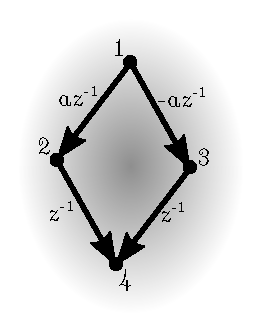
\includegraphics[width=\linewidth]{example1.pdf}
    \caption{Example multiple path cancellation: $j \in \anc{i} \nRightarrow j \pwgc i$}
    \label{fig:diamond_cancellation}
  \end{subfigure}
  \begin{subfigure}[b]{0.35\textwidth}
    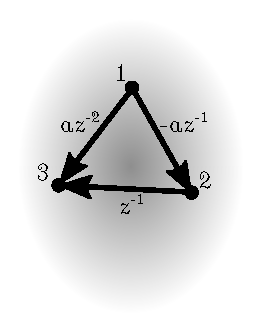
\includegraphics[width=\linewidth]{example2.pdf}
    \caption{Example cancellation from time lag: $j \in \pa{i} \nRightarrow j \pwgc i$}
    \label{fig:lag_cancellation}
  \end{subfigure}
\end{figure}

% \begin{example}
%   \label{ex:lag_cancellation}
%   A second example on $n = 3$ nodes is also worth examining, in this case
%   cancellation is a result of differing time lags.

% \begin{equation*}
%   x(t) =
%   \left[
%     \begin{array}{ccc}
%       0 & 0 & 0\\
%       -a & 0 & 0\\
%       0 & 1 & 0\\
%     \end{array}
%   \right] x(t - 1) +
%   \left[
%     \begin{array}{ccc}
%       0 & 0 & 0\\
%       0 & 0 & 0\\
%       a & 0 & 0\\
%     \end{array}
%   \right] x(t - 2) + v(t)
% \end{equation*}

% Then

% \begin{align*}
%   x_2(t) &= v_2(t) - ax_1(t - 1)\\
%   x_3(t) &= v_3(t) + x_2(t - 1) + ax_1(t - 2)\\
%   \Rightarrow x_3(t) &= v_2(t - 1) + v_3(t),
% \end{align*}

% and again $1 \npwgc 3$.
% \end{example}

\subsection{Strongly Causal Graphs}
\label{sec:strongly_causal_graphs}

In this section and the next we will seek to understand when converse
statements of Proposition \ref{prop:ancestor_properties} \textit{do}
hold.  One possibility is to restrict the coefficients of the system
matrix, e.g. by requiring that $B_{ij}(\tau) \ge 0$.  Instead,
we think it more meaningful to focus on the defining feature of
time series networks, that is, the topology of $\gcg$.

\begin{definition}[Strongly Causal]
  \label{def:strongly_causal}
  We will say that a Granger-causality graph $\gcg$ is
  \textit{strongly causal} if there is at most 1 directed path between
  any two nodes.  Strongly Causal Graphs will be referred to as SCGs.
\end{definition}

Examples of strongly causal graphs include directed trees (or
forests), DAGs where each node has at most one parent, and figure
\ref{fig:example_fig3} of this paper.  A complete bipartite graph with
$2n$ nodes is also strongly causal, demonstrating that the number of
edges of such a graph can still scale quadratically with the number of
nodes.  It is evident that the strong causal property is inherited by
subgraphs.

\begin{example}
  Though examples of SCGs are easy to construct in theory, should
  practitioners expect SCGs to arise in application?  While a positive
  answer to this question is not \textit{necessary} for the concept to
  be useful, it is certainly sufficient.  Though the answer is likely
  to depend upon the particular application area, examples appear to
  be available in biology, in particular, the authors of
  \cite{discovering_graphical_Granger_causality_using_the_truncating_lasso_penalty}
  cite an example of the so called ``transcription regulatory network
  of \textit{E.coli}'', and
  \cite{learning_genome_scale_regulatory_networks} study a much larger
  regulatory network of \textit{Saccharomyces cerevisiae}.  These
  networks, which we reproduce\footnote{Figure \ref{fig:gene_network1}
    is reproduced under the Creative Commons Attribution
    Non-Commercial License
    (\url{http://creativecommons.org/licenses/by-nc/2.5}) and Figure
    \ref{fig:gene_network2} under the Creative Commons Attribution
    License (\url{https://creativecommons.org/licenses/by/4.0/})} in
  figure \ref{fig:gene_networks} appear to have at most a small number
  of edges which violate the strong-causality condition.

  \begin{figure}[h]
    \centering
    \caption{Transcription Regulatory Networks}
    \label{fig:gene_networks}
    \begin{subfigure}[b]{0.45\textwidth}
      \caption{\textit{E.Coli} Network of
        \cite{discovering_graphical_Granger_causality_using_the_truncating_lasso_penalty}}
      \label{fig:gene_network1}
      \includegraphics[width=\linewidth, height=\linewidth]{ecoli_regulatory_network.png}
    \end{subfigure}
    \begin{subfigure}[b]{0.45\textwidth}
      \caption{\textit{Saccharomyces cerevisiae} Network of
        \cite{learning_genome_scale_regulatory_networks}}
      \label{fig:gene_network2}
      \includegraphics[width=\linewidth, height=\linewidth]{huge_gene_network.png}
    \end{subfigure}
  \end{figure}
\end{example}

For later use, and to get a feel for the topological implications of
strong causality, we explore a number of properties of such graphs
before moving into the main result of this section.  The following
important property essentially strengthens proposition
\ref{prop:ancestor_properties} for the case of strongly causal graphs.

\begin{proposition}
  \label{prop:sc_graph_common_anc}
  In a strongly causal graph if $j \in \anc{i}$ then any
  $k \in \anc{i} \cap \anc{j}$ is not a confounder, that is,
  the unique path from $k$ to $i$ contains $j$.
\end{proposition}
\begin{proof}
  Suppose that there is a path from $k$ to $i$ which does not contain
  $j$.  In this case, there are multiple paths from $k$ to $i$ (one of
  which \textit{does} go through $j$ since $j \in \anc{i}$) which
  contradicts the assumption of strong causality.
\end{proof}

\begin{corollary}
  \label{cor:parent_corollary}
  If $\gcg$ is a strongly causal DAG then $i \pwgc j$ and $j \in \anc{i}$ are
  \textit{alternatives}, that is $i \pwgc j \Rightarrow j \notin \anc{i}$.
\end{corollary}
\begin{proof}
  Suppose that $i \pwgc j$ and $j \in \anc{i}$.  Then since $\gcg$ is
  acyclic $i \not\in \anc{j}$, and by proposition
  \ref{prop:ancestor_properties} there is some
  $k \in \anc{i}\cap\anc{j}$ which is a confounder.  However, by
  proposition \ref{prop:sc_graph_common_anc} $k$ cannot be a
  confounder, a contradiction.
\end{proof}
% This is a direct proof
  % \begin{proof}
%   Suppose that $\gcg$ is a strongly causal DAG and that we have both
%   $i \pwgc j$ and $j \in \anc{i}$, which implies that
%   $i \not \in \anc{j}$ since $\gcg$ is a DAG.  We will establish the
%   contradiction $i \in \anc{j}$.

%   Since $j \in \anc{i}$ there is a path $\gcgpath{j}{i}$.
%   Moreover, since $i \pwgc j$ by proposition \ref{prop:pwgc_anc} there
%   must be a confounding ancestor $k \in \anc{i} \cap \anc{j}$, where the
%   node $k$ has a path to $j,\ \gcgpath{k}{j}$, as well as a path
%   to $i,\ \gcgpath{k}{i}$.

%   \hl{Double check that the ancestor properties proposition implies
%     that BOTH paths do not contain the other node.}

%   Now, since the graph is strongly causal, the only possible
%   $\gcgpath{k}{i}$ path is the one obtained by concatenating the
%   $\gcgpath{k}{j}$ path with the $\gcgpath{j}{i}$ path.
%   However, this is a contradiction since $k$ is a confounder and
%   should have a $\gcgpath{k}{i}$ path which does not contain $i$.
% \end{proof}
  
\begin{corollary}
  \label{cor:bidirectional_edge}
  If $\gcg$ is a strongly causal DAG such that $i \pwgc j$ and
  $j \pwgc i$, then $i \not\in \anc{j}$ and $j \not\in \anc{i}$.  In
  particular, a pairwise bidirectional edge indicates the absence of
  any edge in $\gcg$.
\end{corollary}
\begin{proof}
  This follows directly from applying proposition
  \ref{cor:parent_corollary} to $i \pwgc j$ and $j \pwgc i$.
% This is a direct proof
% \begin{proof}
  % By way of contradiction, suppose that $i \in \pa{j}$.  We will
  % consider the two possibilities allowed by proposition
  % \ref{prop:ancestor_properties} for $j \pwgc i$.  Firstly
  % $j \in \anc{i}$ is impossible since $\gcg$ is assumed to be acyclic.
  % Secondly, if there is some confounding node
  % $u \in \anc{i} \cap \anc{j}$ with a path
  % $u \rightarrow \cdots \rightarrow j$ which does not contain $i$ we
  % have a contradiction since there must now be multiple
  % $u \rightarrow j$ paths: the aforementioned, and a path
  % $u \rightarrow \cdots \rightarrow i \rightarrow \cdots \rightarrow
  % j$ which \textit{does} contain $i$.  We conclude that $i \in \pa{j}$
  % is impossible, and symmetrically that $j \in \pa{i}$ is as well.
% \end{proof}
\end{proof}

In light of proposition \ref{prop:sc_graph_common_anc}, the following
provides a partial converse to proposition
\ref{prop:ancestor_properties}, and supports the intuition of ``causal
flow'' through paths in $\gcg$.

\begin{proposition}
  \label{prop:pwgc_anc}
  If $\gcg$ is a strongly causal DAG then $j \in \anc{i} \Rightarrow j \pwgc i$.
\end{proposition}
\begin{proof}
  We will show that for some $\psi \in \H_{t - 1}^{(j)}$ we have

  \begin{equation}
    \label{eqn:cond_ortho_proof}
    \inner{\psi - \linE{\psi}{\H_{t - 1}^{(i)}}}{x_i(t) - \linE{x_i(t)}{\H_{t - 1}^{(i)}}} \ne 0
  \end{equation}

  and therefore that $H_t^{(i)} \not\perp\ \H_{t - 1}^{(j)}\ |\ \H_{t - 1}^{(i)}$, which by theorem (\ref{thm:granger_causality_equivalences}) is enough to establish that $j \pwgc i$.

  Firstly, we will establish a representation of $x_i(t)$ that involves $x_j(t)$.  Denote by $a_{r + 1} \rightarrow a_r \rightarrow \cdots \rightarrow a_1 \rightarrow a_0$ with $a_{r + 1} \defeq j$ and $a_0 \defeq i$ the \textit{unique} $\gcgpath{j}{i}$ path in $\gcg$, we will expand the representation of equation (\ref{eqn:parent_expansion}) backwards along this path:

  % Should this be written as a lemma?
  \begin{align*}
    x_i(t) &= v_i(t) + \B_{ii}(z) x_i(t) + \sum_{k \in \pa{i}}\B_{ik}(z) x_k(t)\\
           &= \underbrace{v_{a_0}(t) + \B_{a_0a_0}(z) x_i(t) + \sum_{\substack{k \in \pa{a_0} \\ k \ne a_1}}\B_{a_0 k}(z) x_k(t)}_{\defeq \wtalpha{a_0}{a_1}} + \B_{a_0a_1}(z)x_{a_1}(t)\\
           &= \wtalpha{a_0}{a_1} + \B_{a_0a_1}(z)\big[\wtalpha{a_1}{a_2} + \B_{a_1a_2}(z)x_{a_2}(t) \big]\\
           &\overset{(a)}{=} \sum_{\ell = 0}^r \underbrace{\Big(\prod_{m = 0}^{\ell - 1} \B_{a_m a_{m + 1}}(z) \Big)}_{\defeq F_\ell(z)} \wtalpha{a_\ell}{a_{\ell + 1}} + \Big(\prod_{m = 0}^{r}\B_{a_m a_{m + 1}}(z)\Big)x_{a_{r + 1}}(t)\\
           &= \sum_{\ell = 0}^r F_\ell(z) \wtalpha{a_\ell}{a_{\ell + 1}} + F_{r + 1}(z) x_j(t)
  \end{align*}

  where $(a)$ follows by a routine induction argument and where we define $\prod_{m = 0}^{-1} \bullet \defeq 1$ for notational convenience.

  Using this representation to expand equation (\ref{eqn:cond_ortho_proof}), we obtain the following cumbersome expression:

  \begin{align*}
    &\inner{\psi - \linE{\psi}{\H_{t - 1}^{(i)}}}{F_{r + 1}(z)x_j(t) - \linE{F_{r + 1}(z)x_j(t)}{\H_{t - 1}^{(i)}}}\\
    &- \inner{\psi - \linE{\psi}{\H_{t - 1}^{(i)}}}{\linE{\sum_{\ell = 0}^r F_\ell(z)\wtalpha{a_\ell}{a_{\ell + 1}}}{\H_{t - 1}^{(i)}}}\\
    &+ \inner{\psi - \linE{\psi}{\H_{t - 1}^{(i)}}}{\sum_{\ell = 0}^r F_\ell(z)\wtalpha{a_\ell}{a_{\ell + 1}}}.
  \end{align*}

  Note that by the orthogonality principle, $\psi - \linE{\psi}{\H_{t - 1}^{(i)}} \perp \H_{t - 1}^{(i)}$, the middle term above is $0$.  Choosing now the particular value $\psi = F_{r + 1}(z)x_j(t) \in \H_{t - 1}^{(j)}$ we arrive at

  \begin{align*}
    &\inner{\psi - \linE{\psi}{\H_{t - 1}^{(i)}}}{x_i(t) - \linE{x_i(t)}{\H_{t - 1}^{(i)}}}\\
    &= \E|F_{r + 1}(z)x_j(t) - \linE{F_{r + 1}(z)x_j(t)}{\H_{t - 1}^{(i)}}|^2\\
    &+ \inner{F_{r + 1}(z)x_j(t) - \linE{F_{r + 1}(z)x_j(t)}{\H_{t - 1}^{(i)}}}{\sum_{\ell = 0}^r F_\ell(z) \wtalpha{a_\ell}{a_{\ell + 1}}},
  \end{align*}

  which by the Cauchy-Schwarz inequality is $0$ if and only if

  \begin{equation*}
    \sum_{\ell = 0}^r F_\ell(z) \wtalpha{a_\ell}{a_{\ell + 1}} \overset{\text{a.s.}}{=} \linE{F_{r + 1}(z)x_j(t)}{\H_{t - 1}^{(i)}} - F_{r + 1}(z)x_j(t),
  \end{equation*}

  or by rearranging and applying the representation obtained earlier, if and only if

  \begin{equation*}
    x_i(t) \overset{\text{a.s.}}{=} \linE{F_{r + 1}(z)x_j(t)}{\H_{t - 1}^{(i)}},
  \end{equation*}

  but this is impossible since $x_i(t) \not \in \H_{t - 1}^{(i)}$.
\end{proof}

We immediately obtain the corollary, which we remind the reader is,
surprisingly, not true in a general graph.

\begin{corollary}
  \label{cor:gc_implies_pwgc}
  If $\gcg$ is a strongly causal DAG then $j \gc i \Rightarrow j \pwgc i$.
\end{corollary}

\begin{remark}
  As we have seen and as is true in much of statistics, confounding
  nodes pose challenges for Granger-causality.  However, as opposed to
  Pearl's causal calculus \cite{pearl2000art}, pairwise
  Granger-causality does not suffer any difficulty with so-called
  ``colliders'', that is, the topology $i \rightarrow k \leftarrow j$
  will never result in $i \pwgc j$ or $j \pwgc i$.  This is evidently
  an advantage of the \textit{temporal} nature of Granger-causality -- there is
  no backwards causal flow along the edges of $\gcg$.
\end{remark}

\begin{example}
  As a final remark of this subsection we note that a complete
  converse to proposition \ref{prop:ancestor_properties} is not
  possible without additional conditions.  Consider the ``fork'' system on $3$
  nodes (i.e. $2 \leftarrow 1 \rightarrow 3$) defined by

  \begin{equation*}
    x(t) =
    \left[
      \begin{array}{cccc}
        0 & 0 & 0\\
        a & 0 & 0\\
        a & 0 & 0\\
      \end{array}
    \right] x(t - 1) + v(t).
  \end{equation*}

  In this case, node $1$ is a confounder for nodes $2$ and $3$, but
  $x_3(t) = v_3(t) - v_2(t) + x_2(t)$ and $2 \npwgc 3$ (even
  though $x_2(t)$ and $x_3(t)$ are contemporaneously correlated)

  If we were to augment this system by simply adding an autoregressive
  component (i.e. some ``memory'') to $x_1(t)$ e.g.
  $x_1(t) = v_1(t) + b x_1(t - 1)$ then we \textit{would} have
  $2 \pwgc 3$ since then
  $x_3(t) = v_3(t) + av_1(t - 1) - bv_2(t - 1) + bx_2(t - 1)$.  We
  develop this idea further in the next section.
\end{example}

\subsection{Persistent Systems}
\label{sec:persistent_systems}
In section \ref{sec:strongly_causal_graphs} we obtained a converse to
part $(a)$ of proposition \ref{prop:ancestor_properties} via the
notion of a strongly causal graph topology.  In this section, we
complete a converse by adding the additional requirement we refer to
as ``persistence''.

\begin{definition}[Lag Function]
  Given a causal filter $\B(z) = \sum_{\tau = 0}^\infty b(\tau)z^{-\tau}$
  define 

  \begin{align}
    \tau_0(\B) &= \text{min}\{\tau \in \Z_+\ |\ b(\tau) \ne 0\},\\
    \tau_{\infty}(\B) &= \text{sup}\{\tau \in \Z_+\ |\ b(\tau) \ne 0\}.\\
  \end{align}

  i.e. the ``first'' and ``last'' coefficients of the filter $\B(z)$,
  where $\tau_\infty(\B) \defeq \infty$ if the filter has an infinite
  length, and $\tau_0(\B) \defeq \infty$ if $\B(z) = 0$.
\end{definition}

This interpretation of the following persistence condition is that
each node stores some ``memory'' of the past.

\begin{definition}[Persistent]
  We will say that the process $x(t)$ with Granger-causality graph
  $\gcg$ is \textit{persistent} if for every $i \in [n]$ and every
  $k \in \anc{i}$ we have $\tau_0(\A_{ik}) < \infty$ and $\tau_\infty(\A_{ik}) = \infty$.
\end{definition}

\begin{remark}
  In the context of Granger-causality, ``most'' systems should be
  persistent.  In particular, $\mathsf{\VAR}(p)$ models are likely to
  be persistent since these naturally result in an equivalent
  $\mathsf{MA}(\infty)$ representation, except for the pathological
  case where $\B(z)$ is Nilpotent.

  Moreover, persistence is not the weakest condition necessary for the
  results of this section, the condition
  $\tau_0(\A_{jk}) < \tau_\infty(\A_{ik})$ for each $i, j, k$ such that
  $k \in \anc{i} \cap \anc{j}$ is enough.  The intuition being that nodes
  $i$ and $j$ are not receiving temporally disjoint information from
  $k$.

\end{remark}

\begin{example}
  process $x(t)$ generated by the $\VAR(1)$ model\footnote{Recall that
    any $\VAR(p)$ model with $p < \infty$ can be written as a
    $\VAR(1)$ model, so we lose little generality in considering this
    case.}  having $\B(z) = Bz^{-1}$, we will examine
  conditions that guarantee persistence.  Pick any
  $i \in [n], j \in \anc{i} \setminus \{i\}$, then the stability of
  $B$ allows us to write

  \begin{equation*}
    \A(z) = \sum_{k = 0}^\infty B^k z^{-k},
  \end{equation*}

  whereby we see that $\exists k > 0$ such that $[B^k]_{ij} \ne 0$
  (since $j \in \anc{i}$).  Then consider

  \begin{equation*}
    \begin{aligned}
      e_i^\T B^{rk} e_j &\overset{(a)}{=} \big((P^\T e_i)^\T J^{rk} P^{-1}e_j\big)\\
      &= \tr [(P^\T e_i)^\T J^{rk} P^{-1}e_j]\\
      &\overset{(b)}{=} \tr [(J^{rk}) (v u^\T)],
    \end{aligned}
  \end{equation*}

  where $(a)$ utilizes the Jordan Normal Form of $B$, and $(b)$
  denotes $u = P^\T e_i$ and $v = P^{-1}e_j$.  In order for
  $\tau_\infty(\A_{ij}) < \infty$, there must be some $N > 1$ such
  that $\forall r \ge N$, the above term is $0$.  This may be the case
  for instance if $B$ is a nilpotent matrix.  

  Let us suppose now that $B$ is diagonalizable (i.e. $J$ is a
  diagonal matrix) with at least $2$ distinct eigenvalues; in this
  case $B$ is also \textit{not} nilpotent.  We can then rewrite the
  above as

  \begin{equation*}
    f(r) \defeq \tr [(J^{rk}) (v u^\T)] = \sum_{\nu = 1}^n \lambda_\nu ^{rk} v_\nu u_\nu \defeq \sum_{\nu = 1}^n \lambda_\nu^{rk} \beta_\nu
  \end{equation*}

  where $\lambda_\nu$ denotes the eigenvalues of $B$ and
  $\beta_\nu = u_\nu v_\nu$.  Note that $f(0) = 0$ since $i \ne j$,
  $u$ is a row of $P$ and $v$ is a column of $P^{-1}$.  Moreover,
  $f(1) \ne 0$ by hypothesis.  But, in order for
  $f(r) = 0\ \forall r \ge N$, it would need to be the case that

  \begin{equation*}
    \Dg(\bm{\lambda})^r \bm{\lambda} = Vz
  \end{equation*}

  had a solution in $z$ for every $r \ge N$, where $V$ is an
  $n \times n - 1$ full-rank matrix whose columns span the nullspace of $\beta$,
  and $\bm{\lambda} = (\lambda_1, \ldots, \lambda_n)$. That is,
  iterates of $\Dg(\bm{\lambda})$ applied to $\bm{\lambda}$ would need to remain
  inside $\beta$'s nullspace.  This would imply that

  \begin{equation*}
    VV^\dagger \bm{\lambda}^{r + 1} = \bm{\lambda}^{r + 1},
  \end{equation*}

  i.e. that $\bm{\lambda}^{r + 1}$ is an eigenvector of $VV^\dagger$
  for an infinite number of integers $r$ (the exponentiation is to be
  understood as a pointwise operation).  However, since there can only
  be a finite number of (unit length) eigenvectors, this cannot be the
  case unless every eigenvalue $(\lambda_1, \ldots, \lambda_n)$ were
  equal.

  We see from this example that the collection of $\VAR(1)$ systems
  which are not persistent are pathological, in the sense that their
  system matrices have zero measure when viewed as a subset of $\R^{n^2}$.
\end{example}

\begin{lemma}
  \label{lem:time_lag_cancellation}
  Suppose $v(t)$ is a scalar sequence with unit variance and zero
  autocorrelation and let $\A(z), \B(z)$ be nonzero and strictly
  causal (i.e. $\tau_0(\A) \ge 1$) linear filters.  Then,

  \begin{equation}
    \inner{F(z)\A(z)v(t)}{\B(z)v(t)} = 0\ \forall \text{ strictly causal filters } F(z)
  \end{equation}

  if and only if $\tau_0(\A) \ge \tau_\infty(\B)$.
\end{lemma}
\begin{proof}
  We have

  \begin{align}
    \inner{\A(z)v(t)}{\B(z)v(t)} &= \sum_{\tau = 1}^\infty \sum_{s = 1}^\infty a(\tau)b(s)\E[v(t - s)v(t - \tau)]\\
    &= \sum_{\tau = \text{max}(\tau_0(\A), \tau_0(\B))}^{\text{min}(\tau_\infty(\A), \tau_\infty(\B))} a(\tau) b(\tau)\\
  \end{align}

  due to the uncorrelatedness assumptions on $v(t)$.  This expression
  is $0$ if and only if $\tau_0(\A) \ge 1 + \tau_\infty(\B)$ or if
  $\tau_0(\B) \ge 1 + \tau_\infty(\A)$ or if the coefficients are
  orthogonal along the common support.

  Specializing this fact to $\inner{F(z)\A(z)v(t)}{\B(z)v(t)} = 0$ we
  see that the coefficients cannot be orthogonal for every choice of
  $F$, and that $\text{sup}_F \tau_\infty(F\A) = \infty$, leaving only
  the possibility that

  \begin{align*}
    \tau_0(F\A) \ge 1 + \tau_\infty(\B) \forall F &\overset{(a)}{\iff} \tau_0(\A) \ge 1 + \tau_\infty(\B) - \underset{F}{\text{min }} \tau_0(F)\\
    &\overset{(b)}{\iff} \tau_0(\A) \ge \tau_\infty(\B),
  \end{align*}

  where $(a)$ follows since $\tau_0(F\A) = \tau_0(F) + \tau_0(\A)$,
  and $(b)$ since $\text{min}_F\ \tau_0(F) = 1$.
\end{proof}

\begin{corollary}
  \label{cor:time_lag_cancellation}
  For $k \in \anc{i} \cap \anc{j}$ we have

  \begin{align*}
    \linE{F(z)\A_{jk}(z)v_k(t)}{\H_{t - 1}^{(i)}} &= 0\ \forall \text{ strictly causal } F(z)\\
    \iff \inner{F(z)\A_{jk}(z)v_k(t)}{\A_{ik}(z)v_k(t)} &= 0\ \forall \text{ strictly causal } F(z)\\
    \iff \tau_0(\A_{jk}) \ge \tau_\infty(\A_{ik})
  \end{align*}
\end{corollary}
\begin{proof}
  The final equivalence follows immediately from Lemma \ref{lem:time_lag_cancellation}.  For the first equivalence we have

  \begin{align*}
    \linE{F(z)\A_{jk}(z)v_k(t)}{\H_{t - 1}^{(i)}} &= 0\ \forall \text{ strictly causal } F(z)\\
    \iff \inner{F(z)A_{jk}(z)v_k(t)}{x_i(t - \tau)} &= 0\ \forall \tau \ge 1, \text{ strictly causal } F(z),
  \end{align*}

  which can be expanded by equation \eqref{eqn:ancestor_expansion} to
  obtain (after cancelling all ancestors of $i$ other than $k$)

  \begin{equation*}
    \inner{F(z)A_{jk}(z)v_k(t)}{\A_{ik}(z)v_k(t - \tau)} = 0\ \forall \tau \ge 1, \text{ strictly causal } F(z),
  \end{equation*}

  which by the Lemma is equivalent to $\tau_0(\A_{jk}) \ge \tau_\infty(\A_{ik})$ as stated.
\end{proof}

\begin{proposition}
  \label{prop:persistence_converse}
  Suppose $\gcg$ is a strongly causal DAG and that $x(t)$ is
  persistent, then if there exists a $k$ which confounds $(i, j)$ we
  have $i \pwgc j$ and $j \pwgc i$.
\end{proposition}
\begin{proof}
  We will show that $j \pwgc i$, the other being symmetric.  First
  note also that by proposition \ref{prop:sc_graph_common_anc} we
  cannot have $i \in \anc{j}$ or $j \in \anc{i}$ and therefore every
  $k \in \anc{i}\cap\anc{j}$ will be a confounder.

  It is sufficient to show that $\exists \psi \in \H_{t - 1}^{(j)}$
  such that

  \begin{equation*}
    \inner{\psi - \linE{\psi}{\H_{t - 1}^{(i)}}}{x_i(t) - \linE{x_i(t)}{\H_{t - 1}^{(i)}}} \ne 0.
  \end{equation*}

  To this end, let $F(z)$ be an arbitrary but strictly causal linear
  filter.  We apply equation \eqref{eqn:ancestor_expansion} to
  $x_i(t)$ and $\psi \defeq F(z)x_j(t)$:

  \begin{align*}
    &\inner{\psi - \linE{\psi}{\H_{t - 1}^{(i)}}}{x_i(t) - \linE{x_i(t)}{\H_{t - 1}^{(i)}}}\\
    &\overset{(a)}{=} \inner{\psi - \linE{\psi}{\H_{t - 1}^{(i)}}}{\A_{ii}(z)v_i(t) + \sum_{k \in \anc{i}}\A_{ik}(z)v_k(t)}\\
    &\overset{(b)}{=} \inner{\sum_{k \in \anc{j}}\big(F(z)\A_{jk}(z)v_k(t) - \linE{F(z)\A_{jk}(z)v_k(t)}{\H_{t - 1}^{(i)}}\big)}{\A_{ii}(z)v_i(t) + \sum_{k \in \anc{i}}\A_{ik}(z)v_k(t)}\\
    &\overset{(c)}{=} \sum_{k \in \anc{i}\cap\anc{j}}\Big(\inner{F(z)\A_{jk}(z)v_k(t)}{\A_{ik}(z)v_k(t)} - \inner{\linE{F(z)\A_{jk}(z)v_k(t)}{\H_{t - 1}^{(i)}}}{\A_{ii}v_i(t)}\\
    &- \sum_{\ell \in \anc{i}}\inner{\linE{F(z)\A_{jk}(z)v_k(t)}{\H_{t - 1}^{(i)}}}{\A_{i\ell}(z)v_\ell(t)}\Big)
  \end{align*}

  where in $(a)$ we have removed the $\linE{x_i(t)}{\H_{t - 1}^{(i)}}$
  term via the orthogonality principle, in $(b)$ there is no
  $F(z)\A_{jj}(z)v_j(t)$ term since due to $j \not\in \anc{i}$ it is
  orthogonal to $\H_t^{(i)}$.  Finally, $(c)$ follows by applying
  orthogonality properties of $v(t)$, as well as the fact that
  $\linE{F(z)\A_{jk}(z)v_k(t)}{\H_{t - 1}^{(i)}} = 0$ for
  $k \not \in \anc{i}$.  Note that
  $\linE{F(z)\A_{jk}(z)v_k(t)}{\H_{t - 1}^{(i)}} \in \H_{t - 1}^{(i)}$
  and thence there is in general no cancellation in the final term
  above for $\ell \in \anc{i}$.

  \todo{This is clearly not immediately evident}

  This is $0$ for every $F$ if and only if for all $F$ and
  $\forall k \in \anc{i} \cap \anc{j}$ we have
  $$\linE{F(z)\A_{jk}(z)v_k(t)}{\H_{t - 1}^{(i)}} = 0$$ and
  $$\inner{F(z)\A_{jk}(z)v_k(t)}{\A_{ik}(z)v_k(t)} = 0,$$ which by
  Corollary \ref{cor:time_lag_cancellation} occurs if and only if
  $\tau_0(\A_{jk}) \ge \tau_\infty(\A_{ik})$, which is impossible since by persistence
  $\tau_0(\A_{jk}) < \infty$ and  $\tau_\infty(\A_{ik}) = \infty$.
\end{proof}

\subsection{Recovering $\gcg$ via Pairwise Tests}
\label{sec:pairwise_algorithm}
In this section we will show that if the $\gcg$ of a persistent
process is a strongly causal DAG, then it is possible to recover
$\gcg$ via pairwise tests alone.  This is the main conclusion of the
theoretical analysis in this paper.

\begin{theorem}[Pairwise Recovery]
  \label{thm:scg_recovery}
  If the Granger-causality graph $\gcg$ for persistent process $x(t)$
  is a strongly causal DAG then $\gcg$ can be inferred from pairwise
  causality tests.  The procedure can be carried out, assuming
  we have an oracle for pairwise causality, via Algorithm
  (\ref{alg:pwgr}).

  \begin{algorithm}
    \SetKwInOut{Input}{input}
    \SetKwInOut{Output}{output}
    \SetKwInOut{Initialize}{initialize}
    \DontPrintSemicolon

    \BlankLine
    \caption{Pairwise Graph Recovery}
    \label{alg:pwgr}
    % \TitleOfAlgo{Pairwise Graph Recovery}
    \Input{Pairwise Granger-causality relations between a persistent
      process of dimension $n$ whose joint Granger-causality
      relations are known to form a strongly causal DAG $\gcg$.}
    \Output{Edges $\gcge = \{(i, j) \in [n] \times [n]\ |\ i \gc j \}$ of
      the graph $\gcg$.}
    \Initialize{$S_0 = [n]$  \texttt{\# unprocessed nodes}\\
      $E_0 = \emptyset$  \texttt{\# edges of }$\gcg$\\
      % $P_0 = \emptyset$  \texttt{\# layer by layer driving nodes}\\
      $k = 1$ \texttt{\# a counter used only for notation}}
    \BlankLine
    $W \leftarrow \{(i, j)\ |\ i \pwgc j, j \npwgc i\}$  \texttt{\# candidate edges}\\
    $P_0 \leftarrow \{i \in S_0\ |\ \forall s \in S_0\ (s, i) \not\in W\}$  \texttt{\# parent-less nodes}\\
    \While{$S_{k - 1} \ne \emptyset$}{
      $S_k \leftarrow S_{k - 1} \setminus P_{k - 1}$ \texttt{\# remove nodes with depth }$k - 1$\\
      $P_k \leftarrow \{i \in S_k\ |\ \forall s \in S_k\ (s, i) \not\in W\}$   \texttt{\# candidate children of }$P_{k - 1}$\\
      \;

      $D_{k0} \leftarrow \emptyset$\\
      \For{$r = 1, \ldots, k$} 
      {
        $Q \leftarrow E_{k - 1} \cup \big(\bigcup_{\ell = 0}^{r - 1} D_{k\ell}\big)$ \texttt{\# currently known edges}\\
        $D_{kr} \leftarrow \{(i, j) \in P_{k - r} \times P_k\ |\ (i, j) \in W,\ \text{no } \gcgpath{i}{j} \text{ path in } Q\}$
        % $E_k \leftarrow E_{k - 1} \cup D_{kr}$ \texttt{\# add edges to }$E_k$ \label{alg:inner_loop_end}\\
        % $W_{k + 1} \leftarrow W_k \setminus D_{kr}$  \texttt{\# remove edges from consideration}\\
      }
      $E_k \leftarrow E_{k - 1} \cup \big(\bigcup_{r = 1}^k D_{kr}\big)$ \texttt{\# update } $E_k$ \texttt{ with new edges}\\
      % \label{alg_line:inner_loop_end}\\
      % $W_{k + 1} \leftarrow W_k \setminus \big(\bigcup_{r = 0}^k D_{kr}\big)$  \texttt{\# remove edges from consideration}\\
      \;
      $k \leftarrow k + 1$
    }
    \Return{$E_{k - 1}$}
  \end{algorithm}
\end{theorem}

We will shortly prove the theorem by establishing the correctness of
algorithm (\ref{alg:pwgr}).  The idea is to iteratively ``peel away
layers'' of nodes by removing the nodes that have no parents
remaining, which always exist since the graph is acyclic.  The
requirement of strong causality ensures that all actual edges of
$\gcg$ manifest in some way as pairwise relations (by proposition
\ref{prop:pwgc_anc}), and the requirement of persistence allows
confounding to be eliminated by removing bidirectional edges.  Without
persistence, each confounded pair would give rise to $4$ possible
pairwise topologies consistent with $\gcg$, one for each type of
pairwise edge (no edge, unidirectional, bidirectional).

\begin{example}
  The set $W$ collects ancestor relations in $\gcg$ (see Lemma
  \ref{lem:W_subset_E}).  In reference to figure
  \ref{fig:example_fig3}, each of the solid black edges, as well as
  the dotted red edges will be included in $W$, but \textit{not} the
  bidirectional green dash-dotted edges, which we are able to exclude
  by appealing to Corollary \ref{cor:bidirectional_edge}.  The
  groupings $P_0, \ldots, P_3$ are also indicated in figure
  \ref{fig:example_fig3}.

  The algorithm proceeds first with the parentless nodes $1, 2$ on the
  initial iteration where the edge $(1, 3)$ is added to $E$.  On the
  next iteration, the edges $(3, 4), (2, 4), (3, 5)$ are added, and
  the false edges $(1, 4), (1, 5)$ are excluded due to the paths
  $1 \rightarrow 3 \rightarrow 4$ and $1 \rightarrow 3 \rightarrow 5$
  already being present.  Finally, edge $(4, 6)$ is added, and the false
  $(1, 6), (3, 6), (2, 6)$ edges are similarly excluded due to the
  ordering of the inner loop.
  
  \begin{figure}
    \centering
    \caption{Example graph for Algorithm \ref{alg:pwgr}}
    \footnotesize{Black arrows indicate true parent-child
      relations.  Red dotted arrows indicate pairwise causality (due to
      non-parent relations), green dash-dotted arrows indicate
      bidirectional pairwise causality (due to the confounding node
      $1$).  Blue groupings indicate each $P_k$ in Algorithm
      \ref{alg:pwgr}.}
    \label{fig:example_fig3}
    
    \begin{subfigure}[b]{0.45\textwidth}
      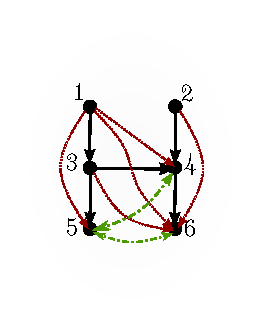
\includegraphics[width=\linewidth]{example_algorithm.pdf}
    \end{subfigure}
    \begin{subfigure}[b]{0.45\textwidth}
      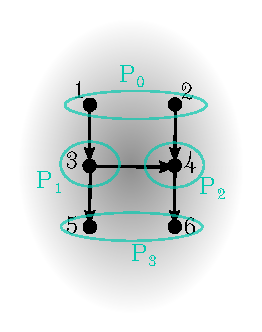
\includegraphics[width=\linewidth]{example_algorithm2.pdf}
    \end{subfigure}
  \end{figure}

  That we need to proceed backwards through $P_{k - r}$ as in the
  inner loop of on $r$ can also be seen from this example, where if
  instead we simply added the set

  \begin{equation*}
    D_k' = \{(i, j) \in \Big(\bigcup_{r = 1}^k P_{k - r}\Big) \times P_k\ |\ i \pwgc j \}
  \end{equation*}

  to $E_k$ then we would infer the false positive edge
  $1 \rightarrow 4$.  Moreover, the same example shows that simply
  using the set

  \begin{equation*}
    D_k'' = \{(i, j) \in P_{k - 1} \times P_k\ |\ i \pwgc j \}  ,
  \end{equation*}

  causes the edge $1 \rightarrow 3$ to be missed.
\end{example}

Our proof proceeds in 5 steps stated formally as lemmas.  Firstly, we
characterize the sets $W$ and $P_k$.  Then we establish a correctness
result for the inner loop on $r$, a correctness result for the outer
loop on $k$, and finally that the algorithm terminates in a finite
number of steps.

\begin{lemma}[$W$ Represents Ancestor Relations]
  \label{lem:W_subset_E}
  In Algorithm \ref{alg:pwgr} we have
  $(i, j) \in W$ if and only if $i \in \anc{j}$.  In particular,
  $W \subseteq \gcge$.
\end{lemma}
\begin{proof}
  Let $j \in [n]$ and suppose that $i \in \anc{j}$.  Then $i \pwgc j$
  by Proposition \ref{prop:pwgc_anc}.  Proposition
  \ref{prop:sc_graph_common_anc} ensures that $(i, j)$ are not
  confounded and Corollary \ref{cor:parent_corollary} that
  $j \not\in \anc{i}$ so $j \npwgc i$ and thence by Proposition
  \ref{prop:ancestor_properties} $(i, j) \in W$.

  Conversely, suppose $(i, j) \in W$.  Then since $j \npwgc i$
  Proposition \ref{prop:persistence_converse} ensures that $(j, i)$
  are not confounded and so by Proposition \ref{prop:ancestor_properties}
  we must have $i \in \anc{j}$.
\end{proof}

\begin{definition}[Depth]
  For our present purposes we will define the \textit{depth} $d(j)$ of
  a node $j$ in $\gcg$ to be the length of the \textit{longest} path
  from a node in $P_0$ to $j$, where $d(j) = 0$ if $j \in P_0$.  It is
  apparent that such a path will always exist.  For example, in Figure
  \ref{fig:example_fig3} we have $d(3) = 1$ and $d(4) = 2$.
\end{definition}

\begin{lemma}[Depth Characterization of $P_k$]
  \label{lem:depth_lemma}
  $i \in P_k \iff d(i) = k$ and $j \in S_k \iff d(j) \ge k$.
\end{lemma}
\begin{proof}
  We proceed by induction, noting that $P_0$ is non-empty since $\gcg$
  is acyclic and therefore $\gcg$ contains nodes without parents.  The
  base case $i \in P_0 \iff d(i) = 0$ is by definition, and
  $j \in S_0 \iff d(j) \ge 0$ is trivial since $S_0 = [n]$.  So
  suppose that the lemma is true up to $k - 1$.

  ($i \in P_k \implies d(i) = k$): Let $i \in P_k$.  Suppose that
  $d(i) \ge k + 1$, then $\exists j \in \pa{i}$ such that
  $j \not\in \cup_{r \ge 1}P_{k - r}$ (otherwise $d(i) \le k$), this
  implies that $j \in S_k$ with $(j, i) \in W$ (by Lemma
  \ref{lem:W_subset_E}) which is not possible due to the construction of
  $P_k$ and therefore $d(i) \le k$.  Moreover,
  $P_k \subseteq S_k \subseteq S_{k - 1}$ implies that
  $d(i) \ge k - 1$ by the induction hypothesis, but if $d(i) = k - 1$
  then $i \in P_{k - 1}$ again by induction which is impossible since
  $i \in P_k$ and therefore $d(i) = k$.

  ($s \in S_k \implies d(s) \ge k$): Let
  $s \in S_k \subseteq S_{k - 1}$.  We have by induction that
  $d(s) \ge k - 1$, but again by induction (this time on $P_{k - 1}$)
  we have $d(s) \ne k - 1$ since $S_k = S_{k - 1} \setminus P_{k - 1}$
  and therefore $d(s) \ge k$.

  ($d(i) = k \implies i \in P_k$): Suppose $i \in [n]$ is such that
  $d(i) = k$.  Then $i \in S_{k - 1}$ by the hypothesis, but also
  $i \not\in P_{k - 1}$ so then
  $i \in S_k = S_{k - 1} \setminus P_{k - 1}$ and thus $d(i) \ge k$.
  Now, recalling the definition of $P_k$

  \begin{equation*}
    P_k = \{i \in S_k\ |\ \forall s \in S_k\ (s, i) \not\in W \},
  \end{equation*}

  if $s \in S_k$ is such that $(s, i) \in W$ then $s \pwgc i$ and
  $i \npwgc s$ so that by persistence and Proposition
  \ref{prop:persistence_converse} there cannot be a confounder of
  $(s, i)$ (otherwise $i \pwgc s$) so then by Proposition
  \ref{prop:ancestor_properties} we have $s \in \anc{i}$.  We have
  shown that $s \in S_k \implies d(s) \ge k$ and so we must have
  $d(i) > k$, a contradiction, thence $s \not\in \anc{i}$,
  $s \npwgc i$, $(s, i) \not\in W$ and $i \in P_k$.

  ($d(j) \ge k \implies j \in S_k$): Let $j \in [n]$ such that
  $d(j) \ge k$, then by induction we have $j \in S_{k - 1}$.  This
  implies by the construction of $S_k$ that $j \not\in S_k$ only if
  $j \in P_{k - 1}$, but we have shown that this only occurs when
  $d(j) = k - 1$, but $d(j) > k - 1$ so $j \in S_k$.
\end{proof}

\begin{lemma}[Inner Loop]
  \label{lem:inner_loop_lemma}
  Fix an integer $k \ge 1$ and suppose that $(i, j) \in E_{k - 1}$ if
  and only if $(i, j) \in \gcge$ and $d(j) \le k - 1$.  Then, we have
  $(i, j) \in D_{kr}$ if and only if $(i, j) \in \gcge $, $d(j) = k$,
  and $d(i) = k - r$.
\end{lemma}
\begin{proof}
  We prove by induction on $r$, keeping in mind the results of Lemmas
  \ref{lem:W_subset_E} and \ref{lem:depth_lemma}.  For the base case,
  let $r = 1$ and suppose that $(i, j) \in \gcge$ with $d(j) = k$ and
  $d(i) = k - 1$.  Then, $(i, j) \in W$ and by our assumptions on
  $E_{k - 1}$ there is no $\gcgpath{i}{j}$ path in $E_{k - 1}$
  and therefore $(i, j) \in D_{k1}$.  Conversely, suppose that
  $(i, j) \in D_{k1}$.  Then, $d(i) = k - 1$ and $d(j) = k$ which, since
  $(i, j) \in W \implies i \in \anc{j}$ implies that
  $i \in \pa{j}$ and $(i, j) \in \gcge$.

  Now, fix $r > 1$ and suppose that the result holds up to $r - 1$.
  Let $(i, j) \in \gcge$ with $d(j) = k$ and $d(i) = k - r$.  Then,
  $(i, j) \in W$ and by induction and strong causality there cannot
  already be an $\gcgpath{i}{j}$ path in
  $E_{k - 1} \cup \big(\bigcup_{\ell = 0}^{r - 1} D_{kr}\big)$,
  therefore $(i, j) \in D_{kr}$.  Conversely, suppose
  $(i, j) \in D_{kr}$.  Then we have $d(i) = k - r$, $d(j) = k$, and
  $i \in \anc{j}$.  Suppose by way of contradiction that
  $i \not\in \pa{j}$, then there must be some $u \in \pa{j}$ such that
  $i \in \anc{u}$.  But, this implies that $d(i) < d(u)$ and by
  induction that $(u, j) \in \bigcup_{\ell = 1}^{r - 1}D_{k\ell}$.
  Moreover, since $d(u) < k$ (otherwise $d(j) > k$) each edge in
  the $\gcgpath{i}{u}$ path must already be in $E_{k - 1}$, and so
  there must be an $\gcgpath{i}{j}$ path in
  $E_{k - 1}\cup\big(\bigcup_{\ell = 0}^{r - 1}D_{kr}\big)$, which is
  a contradiction since we assumed $(i, j) \in D_{kr}$.  Therefore
  $i \in \pa{j}$ and $(i, j) \in \gcge$.
\end{proof}

\begin{lemma}[Outer Loop]
  \label{lem:outer_loop_lemma}
  We have $(i, j) \in E_k$ if and only if $(i, j) \in \gcge$ and
  $d(j) \le k$.  That is, at iteration $k, E_k$ and $\gcge$ agree on
  the set of edges whose terminating node is at most $k$ steps away
  from $P_0$.
\end{lemma}
\begin{proof}
  We will proceed by induction.  The base case $E_0 = \emptyset$ is
  trivial, so fix some $k \ge 1$, and suppose that the lemma holds for
  all nodes of depth less than $k$.

  Suppose that
  $(i, j) \in E_k = E_{k - 1}\cup \big(\bigcup_{r = 1}^k D_{rk}
  \big)$.  Then clearly there is some $1 \le r \le k$ such that
  $(i, j) \in D_{kr}$ so that by Lemma \ref{lem:inner_loop_lemma} we
  have $(i, j) \in \gcge$ and $d(j) = k$.

  Conversely, suppose that $(i, j) \in \gcge$ and $d(j) \le k$.  If
  $d(j) < k$ then by induction $(i, j) \in E_{k - 1} \subseteq E_k$ so
  suppose further than $d(j) = k$.  Since $i \in \pa{j}$ we must have
  $d(i) < k$ (else $d(j) > k$) and again by Lemma
  \ref{lem:inner_loop_lemma} $(i, j) \in \bigcup_{r = 1}^k D_{kr}$
  which implies that $(i, j) \in E_k$.  The result follows.
\end{proof}

\begin{lemma}[Finite Termination]
  Algorithm \ref{alg:pwgr} terminates and returns $E_{k^\star - 1} = \gcge$
  for some $k^\star \le n$.
\end{lemma}
\begin{proof}
  If $n = 1$, the algorithm is clearly correct, returning on the first
  iteration with $E_1 = \emptyset$.  When $n > 1$ Lemma
  \ref{lem:outer_loop_lemma} ensures that $E_k$ coincides with
  $\{(i, j) \in \gcge\ |\ d(j) \le k\}$ and since $d(j) \le n - 1$ for
  any $j \in [n]$ there is some $k^\star \le n$ such that
  $E_{k^\star - 1} = \gcge$.  We must have $S_{k^\star} = \emptyset$
  since $j \in S_{k^\star} \iff d(j) \ge k^\star$ (if $d(j) > k - 1$ then
  $E_{k^\star - 1} \ne \gcge$) and therefore the algorithm terminates.
\end{proof}

\begin{example}
  We close this section by noting that the conditions of persistence
  and strong causality are only sufficient conditions.  For example,
  the complete directed graph with 2 nodes i.e.

  \begin{equation*}
    B(1) = \left[ \begin{array}{cc} 1/2 & 1 \\ 1 & 1/2 \end{array}\right]
  \end{equation*}

  contains a loop but is pairwise recoverable, though not by algorithm
  (\ref{alg:pwgr}).  Clearly, this example is somewhat artificial
  since when $n = 2$ there is no difference between pairwise
  Granger-causality and joint Granger-causality amongst all series --
  however, one can add any number of nodes having no parents or
  children to a graph containing a length 2 cycle, in which case the
  graph clearly remains pairwise recoverable.
\end{example}

\section{Conclusion}
\label{sec:conclusion}
In this paper we have argued that considering particular topological
properties of Granger-causality networks can provide substantial
insights into the structure of causality graphs with potential for
improvements in causality graph estimation when structural assumptions
are met.  In particular, the notion of a strongly-causal graph has
been exploited to establish conditions under which pairwise causality
testing alone is sufficient for recovering a complete
Granger-causality graph.  Moreover, examples from the literature
suggest that such topological assumptions may be reasonable in some
applications.

We emphasize that the causality graph topology is one of the key
defining features of time series analysis in comparison to standard
multivariate regression and therefore advocate for further study of
how different topological assumptions may impact the recovery of
causality graphs.  For example, are there provable guarantees on the
error rate of PWGC when applied to non strongly-causal graphs?
Computationally, can constraint systems or cunning adaptive weighting
schemes impose useful prior knowledge about graph topology for the
LASSO algorithm?  In another direction, it is known that the more
general notion of transfer entropy reduces to Granger-causality in the
case of Gaussian data \cite{barnett2009granger}, do our results extend
to causality networks defined via transfer entropy?

Due to constraints on space, we report upon details for practical
finite sample implementation as well as more extensive simulation
results and an application to EEG data elsewhere \todo{where?}.

% \bibliography{\string~global_bib.bib}
\bibliography{\string~/Documents/academics/global_academics/global_bib}
\end{document}

%%% Local Variables:
%%% mode: latex
%%% TeX-master: t
%%% End:
